%! Tex program = xelatex
\documentclass{article}
%中文
%\usepackage[UTF8]{ctex}
%数学公式
\usepackage{amsmath,amssymb}
%\usepackage{ntheorem}
%\usepackage{mdframed} %公式框1
% e.g., \newmdtheoremenv{theorem}{Theorem}
\usepackage{amsthm}
%边界
\usepackage[letterpaper,top=1cm,bottom=2cm,left=3cm,right=3cm,marginparwidth=1.75cm]{geometry}%table package
%Table
\usepackage{multirow,booktabs}
\usepackage{makecell}
%字体颜色
\usepackage{color}
\usepackage[dvipsnames]{xcolor}  % 更全的色系
%代码
\usepackage[OT1]{fontenc}
% MATLAB 代码风格
\usepackage[framed,numbered,autolinebreaks,useliterate]{/Users/anye_zhenhaoyu/Desktop/Latex/mcode}
\usepackage{listings}
\usepackage{algorithm}
\usepackage{algorithmic}
\usepackage{pythonhighlight} % Python
%插图
\usepackage{graphicx}
%改变item格式
\usepackage{enumerate}
%物理
\usepackage{physics}
%extra arrows
\usepackage{extarrows}
% caption(居中指令)
%\usepackage[justification=centering]{caption}
\usepackage{caption}
% htpb
\usepackage{stfloats}
% pdf 拼接
\usepackage{pdfpages}
% 超链接url
\usepackage{url}

\def\RR{\mathbb{R}}
\def\ZZ{\mathbb{Z}}
\def\EE{\mathbb{E}}

\def\Trsp#1{#1^{\mathcal{T}}}
\def\LT{\mathcal{L}}

\def\bold#1{\boldsymbol{#1}}
\def\bw{\boldsymbol{\omega}}
\def\ba{\boldsymbol{a}}
\def\bb{\boldsymbol{b}}
\def\bc{\boldsymbol{c}}
\def\bd{\boldsymbol{d}}
\def\be{\boldsymbol{e}}
\def\bf{\boldsymbol{f}}
\def\bg{\boldsymbol{g}}
\def\bh{\boldsymbol{h}}
\def\bt{\boldsymbol{t}}
\def\bu{\boldsymbol{u}}
\def\bv{\boldsymbol{v}}
\def\bx{\boldsymbol{x}}
\def\by{\boldsymbol{y}}
\def\bz{\boldsymbol{z}}

\def\bA{\boldsymbol{A}}
\def\bB{\boldsymbol{B}}
\def\bC{\boldsymbol{C}}
\def\bE{\boldsymbol{E}}
\def\bF{\boldsymbol{F}}
\def\bG{\boldsymbol{G}}
\def\bL{\boldsymbol{L}}
\def\bM{\boldsymbol{M}}
\def\bO{\boldsymbol{O}}
\def\bP{\boldsymbol{P}}
\def\bQ{\boldsymbol{Q}}
\def\bX{\boldsymbol{X}}
\def\bY{\boldsymbol{Y}}

\def\Esolve{\textcolor{blue}{Solve: }}
\def\Eproof{\textcolor{blue}{Proof: }}
\def\case#1{\textcolor{blue}{Case \uppercase\expandafter{\romannumeral#1}: }}

\def\suminf#1{\sum_{#1=-\infty}^{+\infty}}

\newtheorem{lemma}{Lemma}
\newtheorem{theorem}{Theorem}
\newtheorem{defination}{Definition} 

\graphicspath{{figures/}}

\begin{document}
\title{Homework 12}
\author{Zhen}
\maketitle

\section*{Problem 1}

\begin{enumerate}[(a)]
    \item
		By the fact that
		\[
		    \begin{aligned}
				\nabla f(\bx)&=
				\mqty[e^{x_1} & 2e^{x_2} & 2e^{x_3}]^T
				\\
				\nabla^2 f(\bx)&=
				\mbox{diag}(e^{x_1},4e^{x_2},4e^{x_3})
		    \end{aligned}
		\]
		Let $\bx=(x_1,x_2,x_3)$ and $\bd=(d_1,d_2,d_3)$. The KKT system is:
		\[
			\mqty[
				e^{x_1} & 0 & 0 & 1 \\
				0 & 4e^{x_2} & 0 & 1 \\
				0 & 0 & 4e^{x_3} & 1 \\
				1 & 1 & 1 & 0
			]
			\mqty[d_1 \\ d_2 \\ d_3 \\ \lambda]
			=
			-\mqty[e^{x_1} \\ 2e^{x_2} \\ 2e^{x_3} \\ 0]
		\]

		Thus we have $\lambda=-\dfrac{8}{4e^{-x_1}+e^{-x_2}+e^{-x_3}}$.
		
		Finally,
		\[
			d_1=
			\dfrac{4e^{-x_1}-e^{-x_2}-e^{-x_3}}
			{4e^{-x_1}+e^{-x_2}+e^{-x_3}}
		,\]

		\[
			d_2=
			\dfrac{-2e^{-x_1}+3/2e^{-x_2}-1/2e^{-x_3}}
			{4e^{-x_1}+e^{-x_2}+e^{-x_3}}
		\] and
		\[
			d_3=
			\dfrac{-2e^{-x_1}-1/2e^{-x_2}+3/2e^{-x_3}}
			{4e^{-x_1}+e^{-x_2}+e^{-x_3}}
		.\]
    \item
		The output of my code:
		\\
		\texttt{
			iteration 0: [0. 1. 0.]\\
			iteration 1: [ 0.55783402  0.55270748 -0.1105415 ]\\
			iteration 2: [0.74171111 0.22388047 0.03440841]\\
			iteration 3: [0.83735858 0.09139269 0.07124873]\\
			iteration 4: [0.8464719  0.07685719 0.07667091]\\
			iteration 5: [0.84657358 0.07671322 0.0767132 ]\\
			iteration 6: [0.84657359 0.0767132  0.0767132 ]\\
			optimal value: 4.663287963194248
		}
\end{enumerate}

\newpage
\section*{Problem 2}
\begin{enumerate}[(a)]
    \item
        \[
            \begin{aligned}
				\min_{\bx\in\RR^n}\ \ &
				\bc^T\bx
				-\frac{1}{t}\sum_{i=1}^n\log{x_i}
				\\
				\mbox{s.t.}\ \ &
				\bA\bx=\bb
            \end{aligned}
        \]
    \item
		Let $f(\bx)=\bc^T\bx-\dfrac{1}{t}\sum_{i=1}^n\log{x_i}$. Then we have:
		\[
		    \nabla f(\bx)=\bc-\frac{1}{t}\frac{1}{\bx}
		\]
		where $\dfrac{1}{\bx}=\mqty[\dfrac{1}{x_1},\dfrac{1}{x_2},\dots,\dfrac{1}{x_n}]^T$.

		Also,
		\[
			\nabla^2f(\bx)=\mbox{diag}\qty(\frac{1}{t\bx_1^2},\frac{1}{t\bx_2^2},\dots,\frac{1}{t\bx_n^2})
		.\]
	\item(d)

		Let $\bx=(x_1,x_2,x_3,x_4)$. Then we attain the standard form:
		\[
		    \begin{aligned}
				\min_{\bx}\ \ \ &
				-x_1-3x_2
				\\
				\mbox{s.t.}\ \ \ 
				&
				x_1+x_2+x_3=6
				\\
				&
				x_1-2x_2-x_4=-8
				\\
				&x_1,x_2,x_3,x_4\ge0
		    \end{aligned}
		\]

		The output of ``p2.py'':\\
		\texttt{
			iteration 0: [2. 1. 3. 8.]\\
			iteration 1: [1.63307563 3.90402064 0.46290373 1.82503435]\\
			iteration 2: [1.34600004 4.59597677 0.05802319 0.1540465 ]\\
			iteration 3: [1.3343604  4.65966009 0.00597951 0.01504022]\\
			iteration 4: [1.33343360e+00 4.66596660e+00 5.99794358e-04 1.50040181e-03]\\
			iteration 5: [1.33334334e+00 4.66659667e+00 5.99948876e-05 1.49996563e-04]\\
			iteration 6: [1.33333433e+00 4.66665967e+00 5.99937452e-06 1.49985317e-05]\\
			iteration 7: [1.33333343e+00 4.66666597e+00 5.99939244e-07 1.49984906e-06]\\
			iteration 8: [1.33333334e+00 4.66666660e+00 5.93972887e-08 1.48493250e-07]\\
			iteration 9: [1.33333333e+00 4.66666666e+00 3.99866757e-09 9.99667352e-09]\\
			optimal value: -15.333333320004442
		}
		\begin{figure}[H]
			\centering
			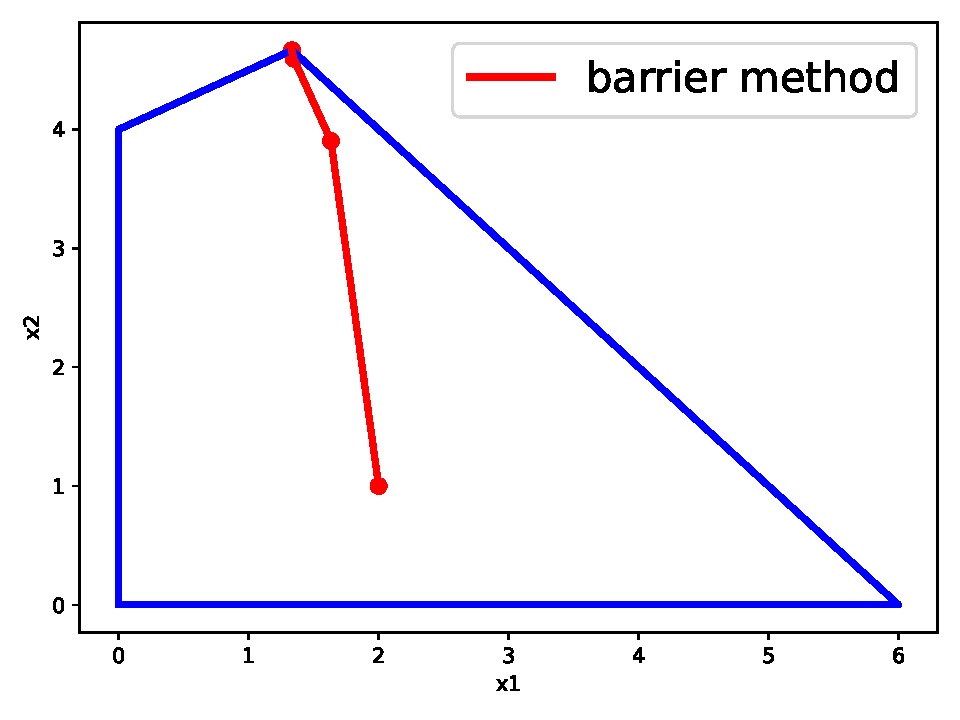
\includegraphics[width=0.6\linewidth]{p2.pdf}
			\caption{The projection of the iterates onto the $x_1,x_2$ coordinates}
		\end{figure}
\end{enumerate}

\section*{Problem 3}

\begin{enumerate}[(a)]
    \item
		Let $\bold{\mu}=\mqty[\mu_1,\mu_2,\mu_3,\mu_4]^T$.
		Then we have:
		\[
		    \begin{aligned}
		        \max_{\bold{\mu}}\ \ 
				&
				\bh^T\bold{\mu}
				\\
				\mbox{s.t.}\ \ 
				&
				\bG^T\bold{\mu}=\bc
				\\
				&
				\bold{\mu}\ge\bold{0}
		    \end{aligned}
		\]
		where 
		\[
			\bG=\mqty[
				-1 & -1 \\
				1 & -2 \\
				1 & 0 \\
				0 & 1
			],\ 
			\bh=\mqty[-6 \\ -8 \\ 0 \\ 0]
			,\ 
			\bc=\mqty[-1 \\ -3]
		\] 
    \item
		Let $\bold{\mu}=\mqty[\mu_1 & \mu_2]$. Then the symmetric dual LP is
		\[
		    \begin{aligned}
		        \max_{\bold{\mu}}\ \ 
				&
				-6\mu_1-8\mu_2
				\\
				\mbox{s.t.}\ \ 
				&
				\mu_1-\mu_2\ge 1
				\\
				&
				\mu_1+2\mu_2\ge 3
				\\
				&
				\mu_1,\mu_2\ge 0
		    \end{aligned}
		\]
	\item
		The dual optimal solution and value:
		\[
			\mu_1=\frac{5}{3},\ \mu_2=\frac{2}{3},\ f'^*=-\frac{46}{3}
		\]
		The primal optimal solution and value:
		\[
			x_1=\frac{4}{3},\ x_2=\frac{14}{3},\ f^*=-\frac{46}{3}
		\]
		\begin{figure}[H]
			\centering
			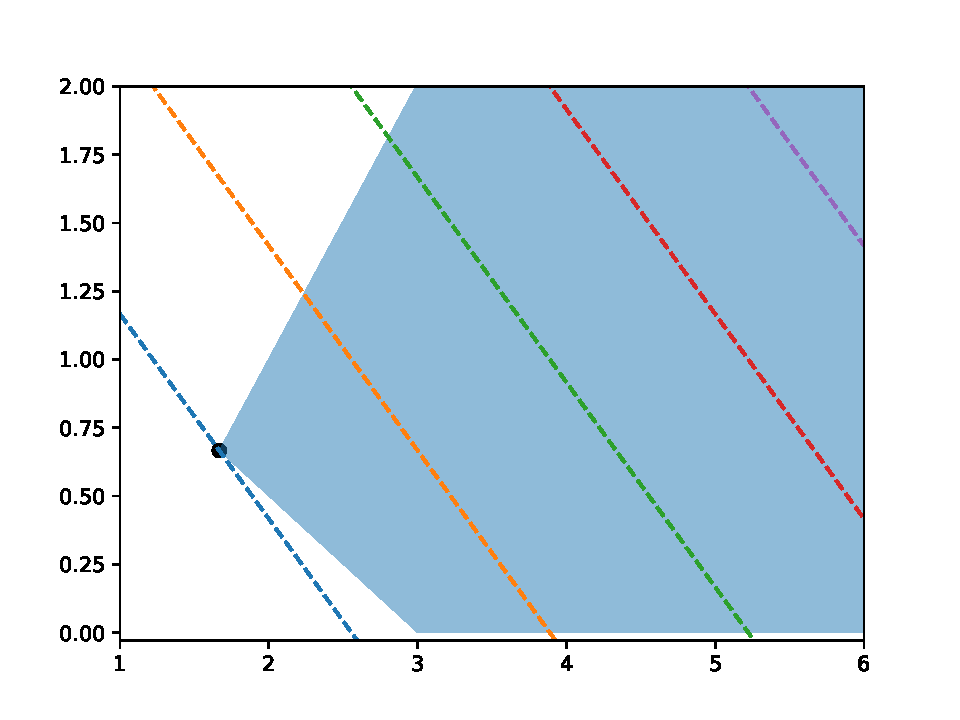
\includegraphics[width=0.5\linewidth]{p3.pdf}
		\end{figure}
	\item
		The output:\\
		\texttt{
			iteration 0: [4. 1. 2. 3.]\\
			iteration 1: [2.1602764  0.54793489 0.61234151 0.25614619]\\
			iteration 2: [1.72344885 0.64915465 0.0742942  0.02175816]\\
			iteration 3: [1.67237818 0.66488395 0.00749423 0.00214608]\\
			iteration 4: [1.66723807e+00 6.66488125e-01 7.49943600e-04 2.14317864e-04]\\
			iteration 5: [1.66672380e+00 6.66648812e-01 7.49918806e-05 2.14267532e-05]\\
			iteration 6: [1.66667238e+00 6.66664881e-01 7.49923738e-06 2.14264427e-06]\\
			iteration 7: [1.66666723e+00 6.66666490e-01 7.42466015e-07 2.12133296e-07]\\
			iteration 8: [1.66666672e+00 6.66666651e-01 6.66555489e-08 1.90444589e-08]\\
			iteration 9: [1.66666667e+00 6.66666666e-01 9.38122456e-10 2.68017088e-10]\\
			dual optimal value: -15.333333335834917
		}
\end{enumerate}

\end{document}

